\let\negmedspace\undefined
\let\negthickspace\undefined
\documentclass[journal]{IEEEtran}
\usepackage[a5paper, margin=10mm, onecolumn]{geometry}
%\usepackage{lmodern} % Ensure lmodern is loaded for pdflatex
\usepackage{tfrupee} % Include tfrupee package

\setlength{\headheight}{1cm} % Set the height of the header box
\setlength{\headsep}{0mm}     % Set the distance between the header box and the top of the text

\usepackage{gvv-book}
%\usepackage{gvv}
\usepackage{cite}
\usepackage{amsmath,amssymb,amsfonts,amsthm}
\usepackage{algorithmic}
\usepackage{graphicx}
\usepackage{textcomp}
\usepackage{xcolor}
\usepackage{txfonts}
\usepackage{listings}
\usepackage{enumitem}
\usepackage{mathtools}
\usepackage{gensymb}
\usepackage{comment}
\usepackage[breaklinks=true]{hyperref}
\usepackage{tkz-euclide} 
\usepackage{listings}
\usepackage{gvv}                                        
\def\inputGnumericTable{}                                 
\usepackage[latin1]{inputenc}                                
\usepackage{color}                                            
\usepackage{array}                                            
\usepackage{longtable}                                       
\usepackage{calc}                                             
\usepackage{multirow}                                         
\usepackage{hhline}                                           
\usepackage{ifthen}                                           
\usepackage{lscape}
\begin{document}

\bibliographystyle{IEEEtran}

\title{1.9.6}
\author{EE25BTECH11017 - Mahesh Chollangi.}
{\let\newpage\relax\maketitle}

\renewcommand{\thefigure}{\theenumi}
\renewcommand{\thetable}{\theenumi}
\setlength{\intextsep}{10pt}

\numberwithin{figure}{enumi}
\renewcommand{\thetable}{\theenumi}

\textbf{Question}:\\
If $\vec{Q}$ = $\brak{0,1}$ is equidistant from $\vec{P}$ = $\brak{5,-3}$ and $\vec{R}$ = $\brak{x,6}$, find the value of x.{\hspace{2cm}} \hfill $\brak{10,2023}$\\


\solution \\

\begin{table}[h!]    
  \centering
  \begin{tabular}{|c|c|c|}
\hline
\textbf{Variable} & \textbf{Description} \\
\hline
$\vec{P}$ & Point $\brak{5,-3}$ \\
\hline
$\vec{Q}$ & Point $\brak{0,1}$ \\
\hline
$\vec{R}$ & Point $\brak{x,6}$ \\
\hline
\end{tabular}
  \caption{Variables Used}
  \label{tab10.5.8.1}
\end{table}

\begin{align}
\vec{P} &= \myvec{5\\-3}, \quad 
\vec{Q} = \myvec{0\\1},  \quad
\vec{R} = \myvec{x\\6}
\end{align}

Given that point $\vec{Q}$ is equidistant from the points $\vec{P}$ and $\vec{R}$, which is given by
\begin{align}
\norm{\vec{Q}-\vec{P}} &= \norm{\vec{Q}-\vec{R}}
\end{align}

Substituting values,
\begin{align}
\norm{\myvec{0\\1}-\myvec{5\\-3}} = \norm{\myvec{0\\1}-\myvec{x\\6}} \\
\norm{\myvec{-5\\4}} = \norm{\myvec{-x\\-5}} \\
\sqrt{(5)^2 + (4)^2} = \sqrt{(x)^2 + (5)^2}\\
\end{align}

Simplifying,
\begin{align}
(5)^2 + (4)^2 &= (x)^2 + (5)^2  \\
(4)^2  &= (x)^2
\end{align}

\begin{align}
\implies x = 4 \quad and \quad x = -4
\end{align}
Hence, the required values of x are :
x = 4 and x = -4
\begin{figure}[H]
\centering
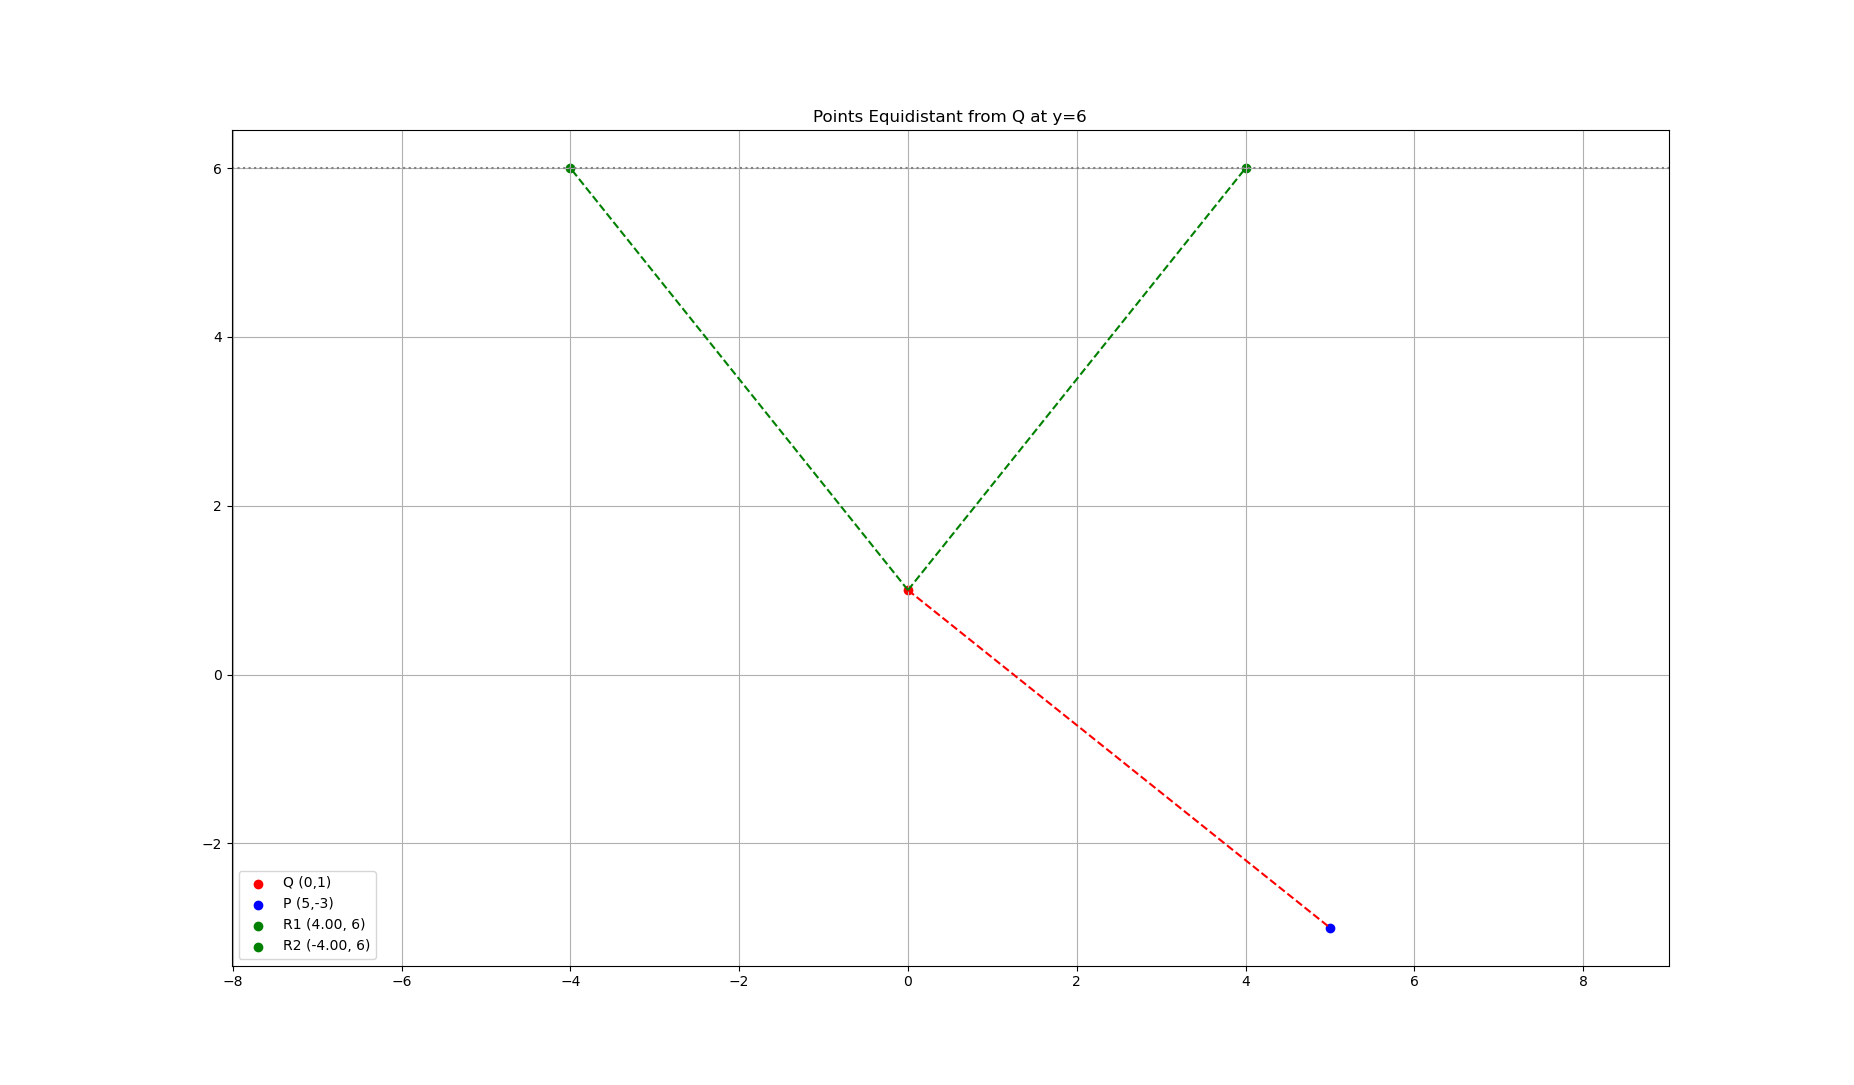
\includegraphics[width=0.75\columnwidth]{Figs/Figure_1.png}
\caption{\centering plot}
\label{fig:placeholder_125}
\end{figure}
\end{document}
